\documentclass[letter,12pt]{article}

%---------------------------------------------------------------
\usepackage{listings} % allow to include nicely formated listings
\usepackage{color}    % we can add color
\usepackage{graphics}
\usepackage{fullpage} % default article style is to greedy about margins
\usepackage{amsmath}
\usepackage{amsthm}
\usepackage{amssymb}
\usepackage{amsfonts}
\usepackage{mathtools}
\usepackage{algorithm}
\usepackage{listings}
%---------------------------------------------------------------

\begin{document}

%---------------------------------------------------------------
\title{Homework report: Assignment III}
\author{Cristian Gonzalez, T00902102\\
Holger Rasmussen, A00922103\\
Barbara Sepic, A00922104,\\
Felix Stahlberg, A00922105
}
\maketitle
\section{Introduction}
This report describes the design rationale, process, experimental results of the Camera Calibration (A) and the Object Detection (B) programs.   As to the work distribution, Barbara and Cristian were responsible for part A.  Felix and Holger are responsible for part B.  
\section{Part A (Camera Calibration)}
\subsection{Problem Statement and Used Resources}
The goal of this assigment is to get familiar the camear model and the meaning of the camera parameters.  In order to achieve this, it was our task to execute a camera calibration and explain the results.  Especially the intrinsic and extrinsic parameters are of interest. 

Resources needed for this task are a camera, a printed out checkerboard and the OpenCV library.  The camera used in the calibration is the a 5 megapixel color camera with auto focus and power LED flash ("HTC desire S" camera).  The dimensions of the checkerboard is as follows:
\begin{itemize}
	\item Board width: 8 squares
	\item Board height: 6 Squares
	\item Square size: 2.5 cm * 2.5 cm
\end{itemize}

For the experiment, 20 images of the checkboard were taken with the specified camera.  Each image was taken at a different angle.  The images and the dimensions of the checkerboard serve as the input for the camera calibration.
\subsection{result}
As a result of the camera calibration, we calculated the following intrinsic parameters, which are displayed in a 3x3 matrix:

\begin{center}
$\begin{bmatrix} [ 2.9072828604088395e+03 & 0& 1.3553413676263517e+03\\ 0 & 2.8931612870671734e+03 & 4.7380351999214878e+02\\0 & 0 &1 \end{bmatrix}$
\end{center}
In order to explain this matrix, the individual parameters are explained as follows:

\begin{itemize}
\item $\gamma = 0$, which means there is no skew between the x-axis and the y-axis
\item $\mu_0 = 1.3553413676263517e+03$, $\nu_0 = 4.7380351999214878e+02$ which are the principal points of the camera, which means the point of where the distortions might start occuring
\item $\alpha_x = 2.9072828604088395e+03$, $\alpha_y= 2.8931612870671734e+03$
both $\alpha_x$ and $\alpha_y$ give a clue to what the focal length is for x and y direction respectively. Focal length is usually multiplied by the pixel length of x and y direction respectively. So it means with these two numbers, we have a good idea how far the objects really are from the image in 2D space.
\end{itemize}

According to the program, the following is the matrix for the distortion:

\begin{center}
$\begin{bmatrix} [$1.9827021688267019e-01$ & $-6.0612987498128668e-01$& $-2.6589049569987616e-02$&$ 8.2291961184871847e-03$ \end{bmatrix}$
\end{center}
Some of the images look almost the same from before the calibration and after the calibration.  One example are the following before and after images:

\begin{figure}[h]
\begin{center}$
\begin{array}{cc}
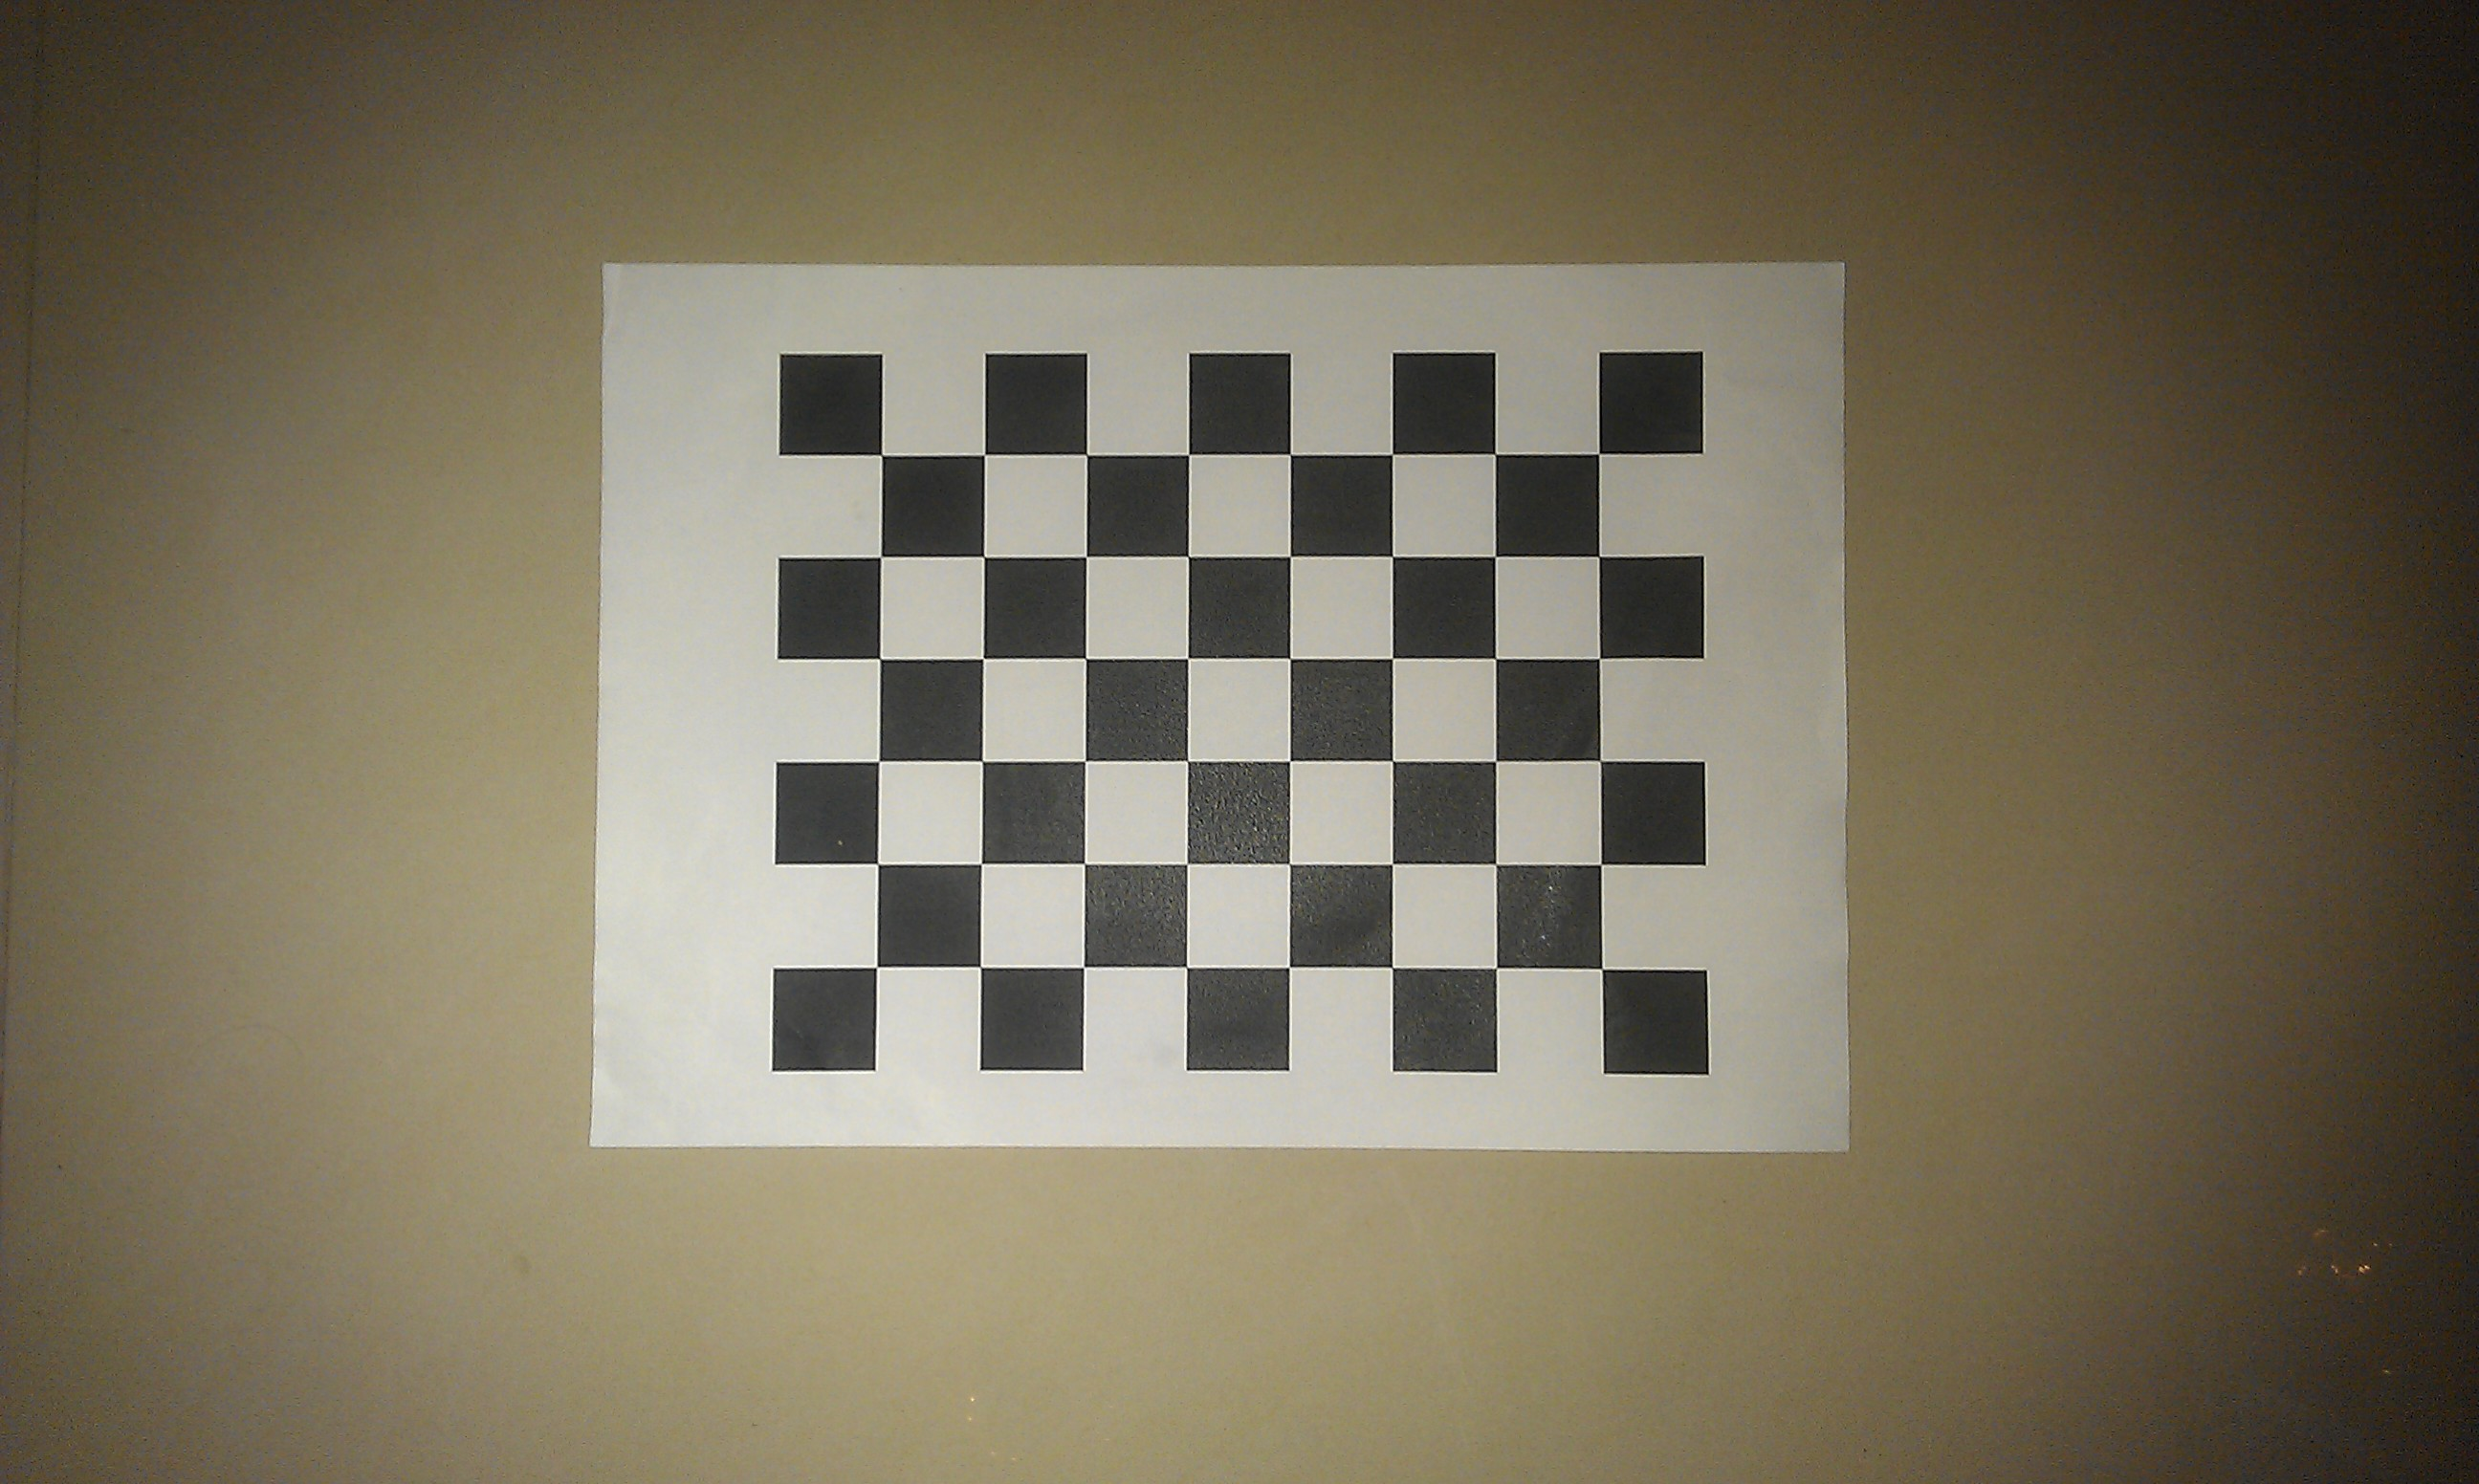
\includegraphics[scale=0.08]{image1.jpg} &
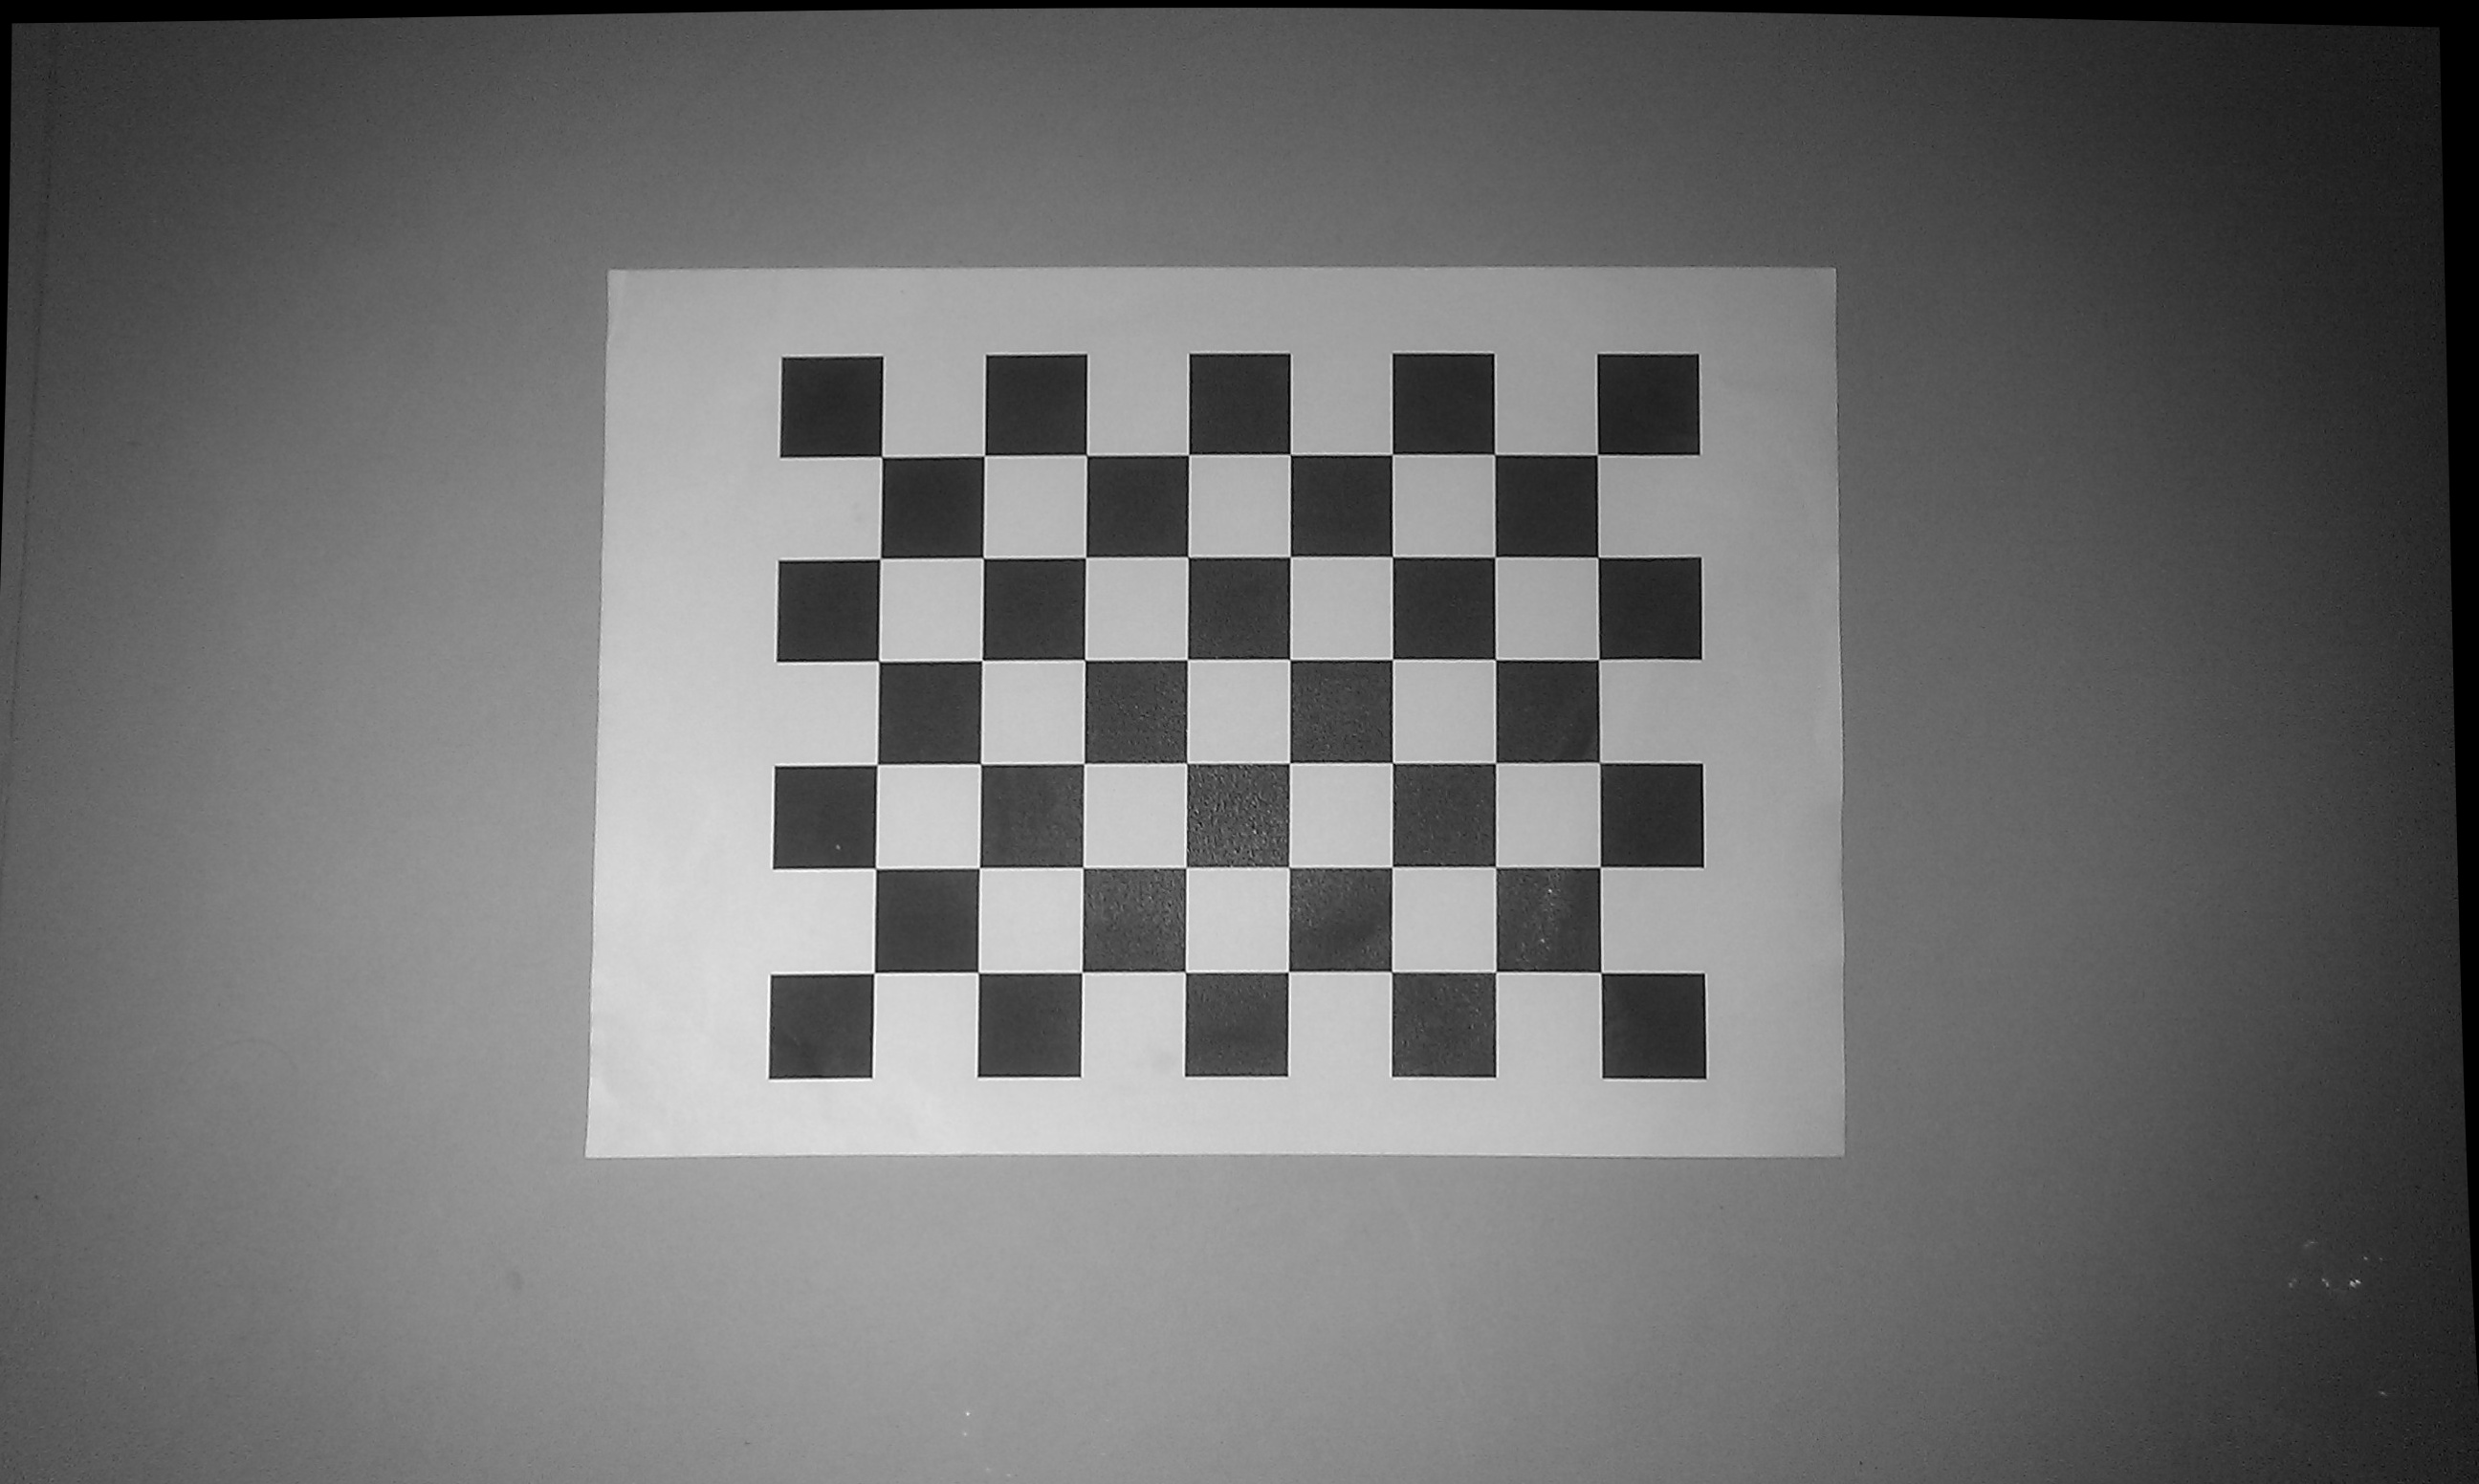
\includegraphics[scale=0.08]{image2.jpg} 
\end{array}$
\end{center}
\caption{The left image is the raw image of the camera.  The right image shows the image after calibration}
\end{figure}

Other pictures are not so nice looking, as the next set of images show.  Some of the reasons for the distortion of the images is because there might be some sort of error in the alignment of the lens or in the distortion of the lens of a camera. It could also be because of the image might be close to the principal point, since the closer the object is from the principal point is, the more noticeable the distortions of an image are noticed, at least based on our observation of the images. 
\begin{figure}[h]
\begin{center}$
\begin{array}{cc}
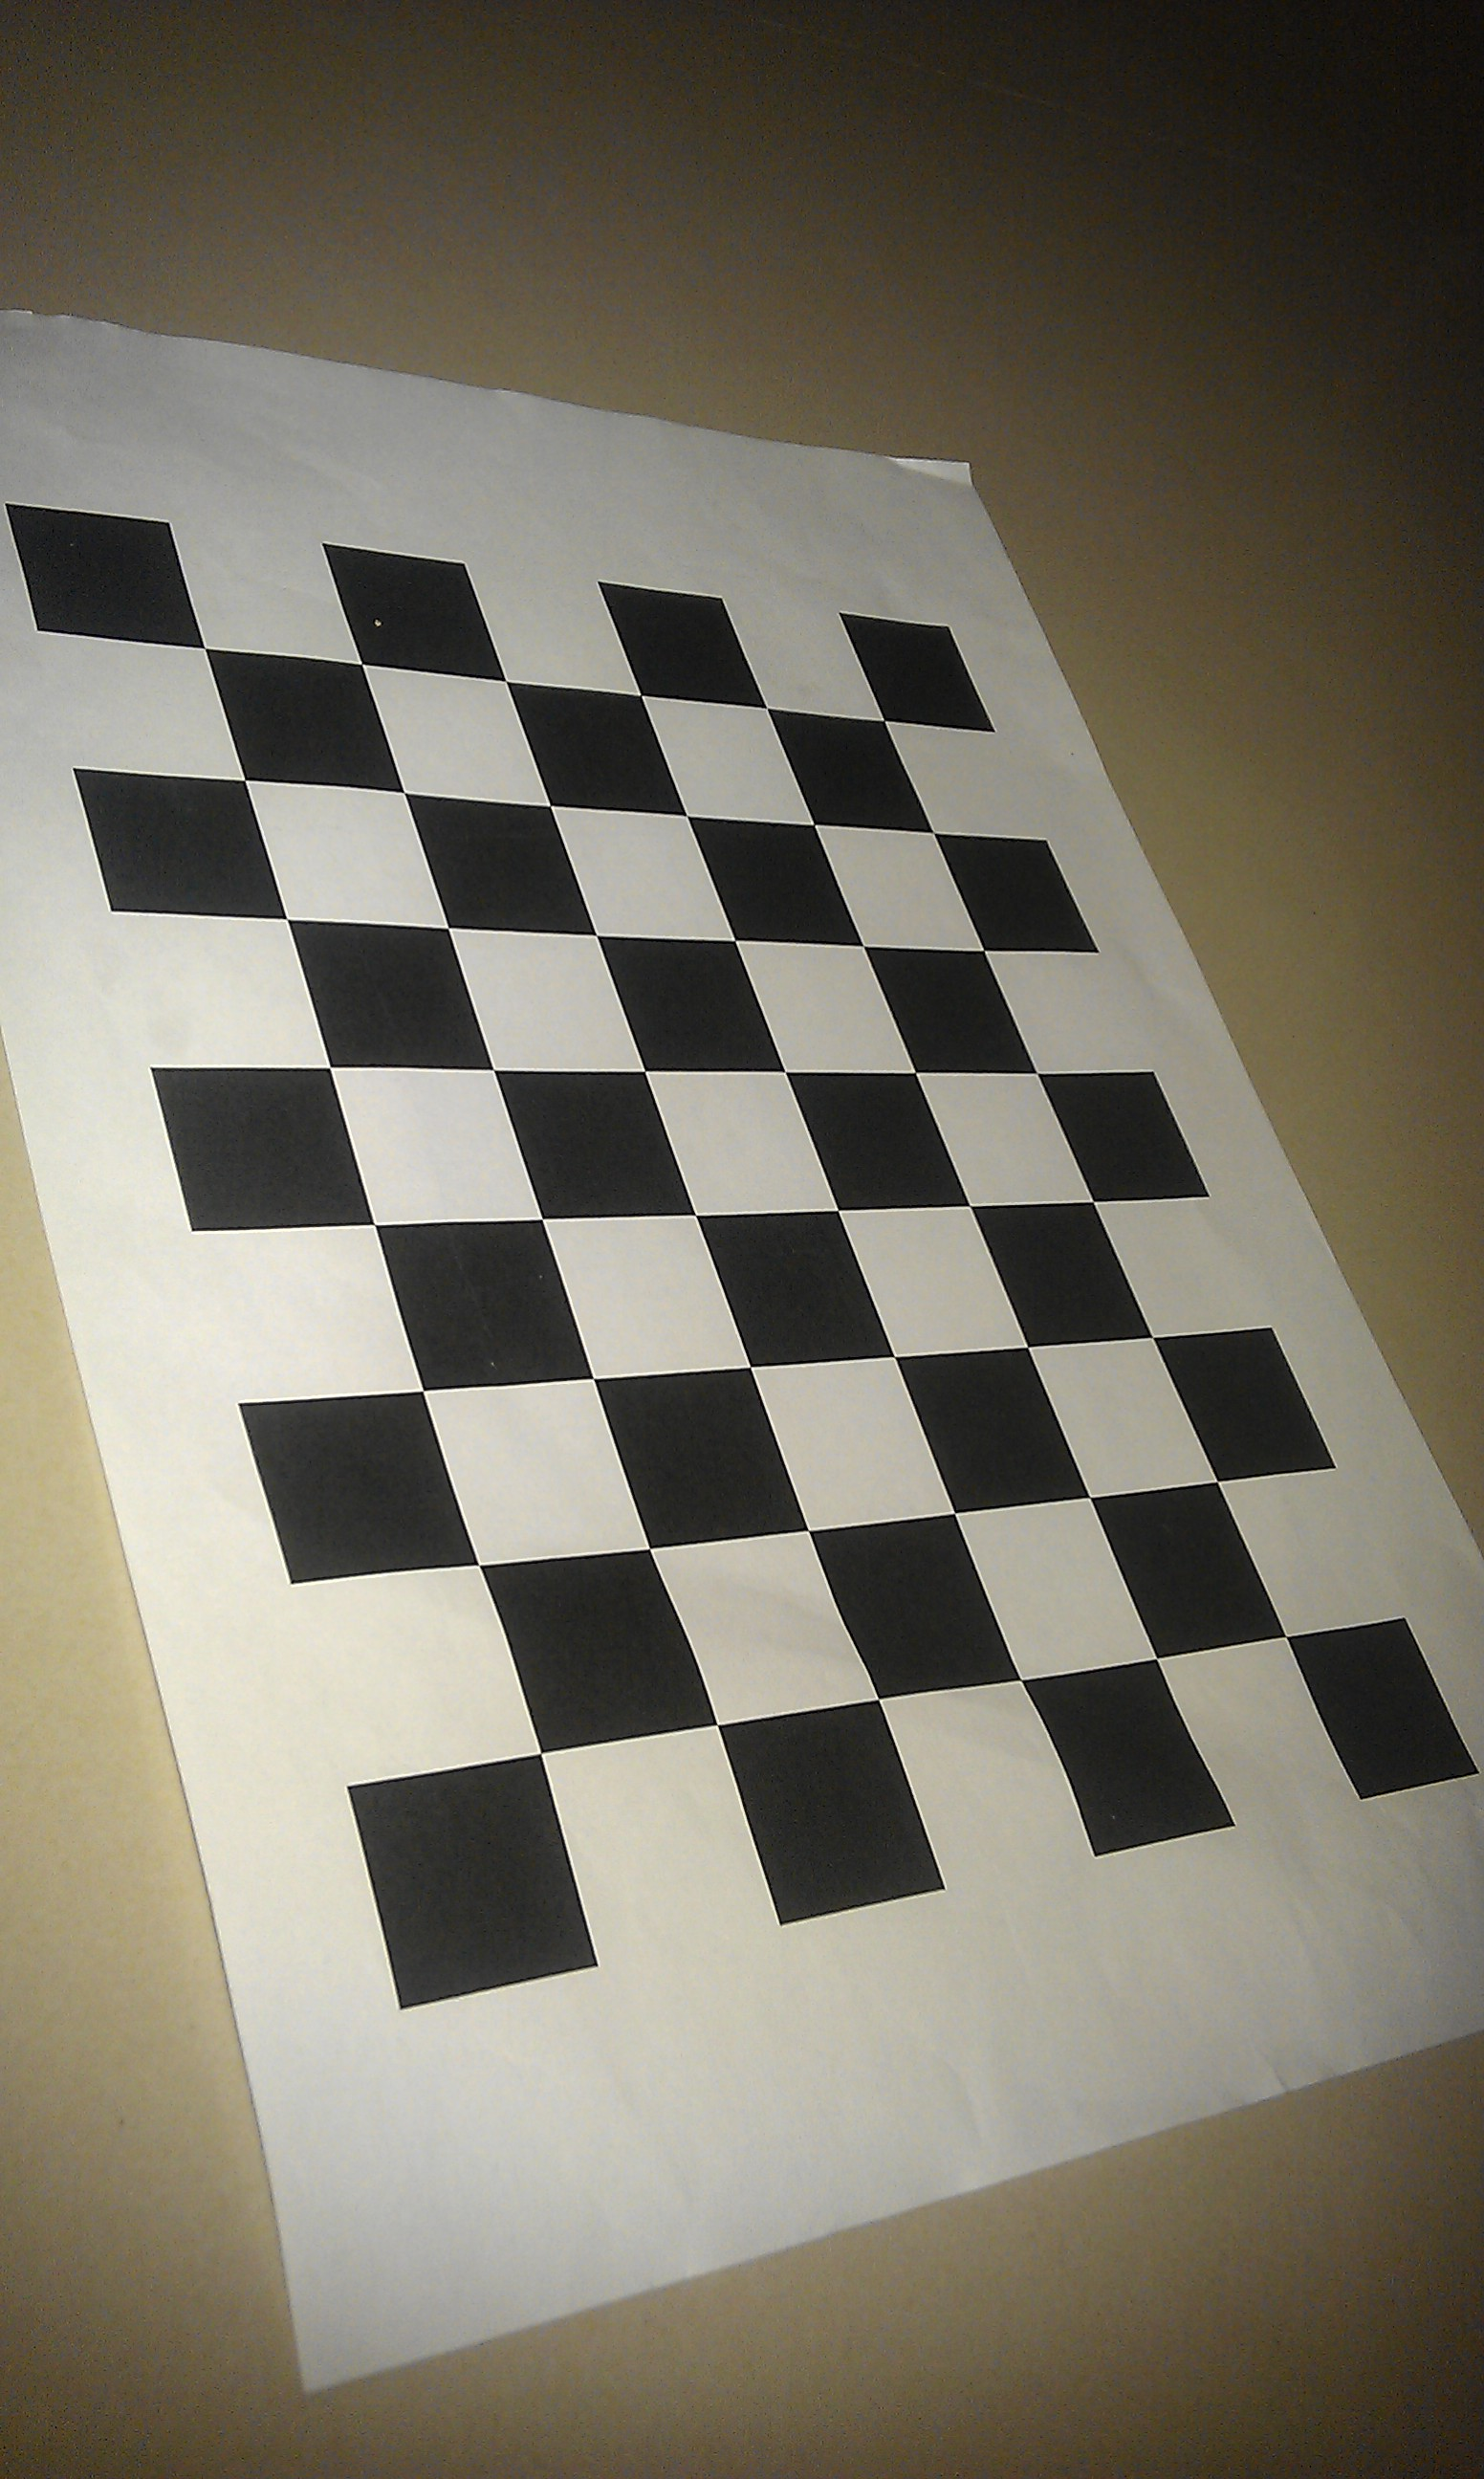
\includegraphics[scale=0.08]{image3.jpg} &
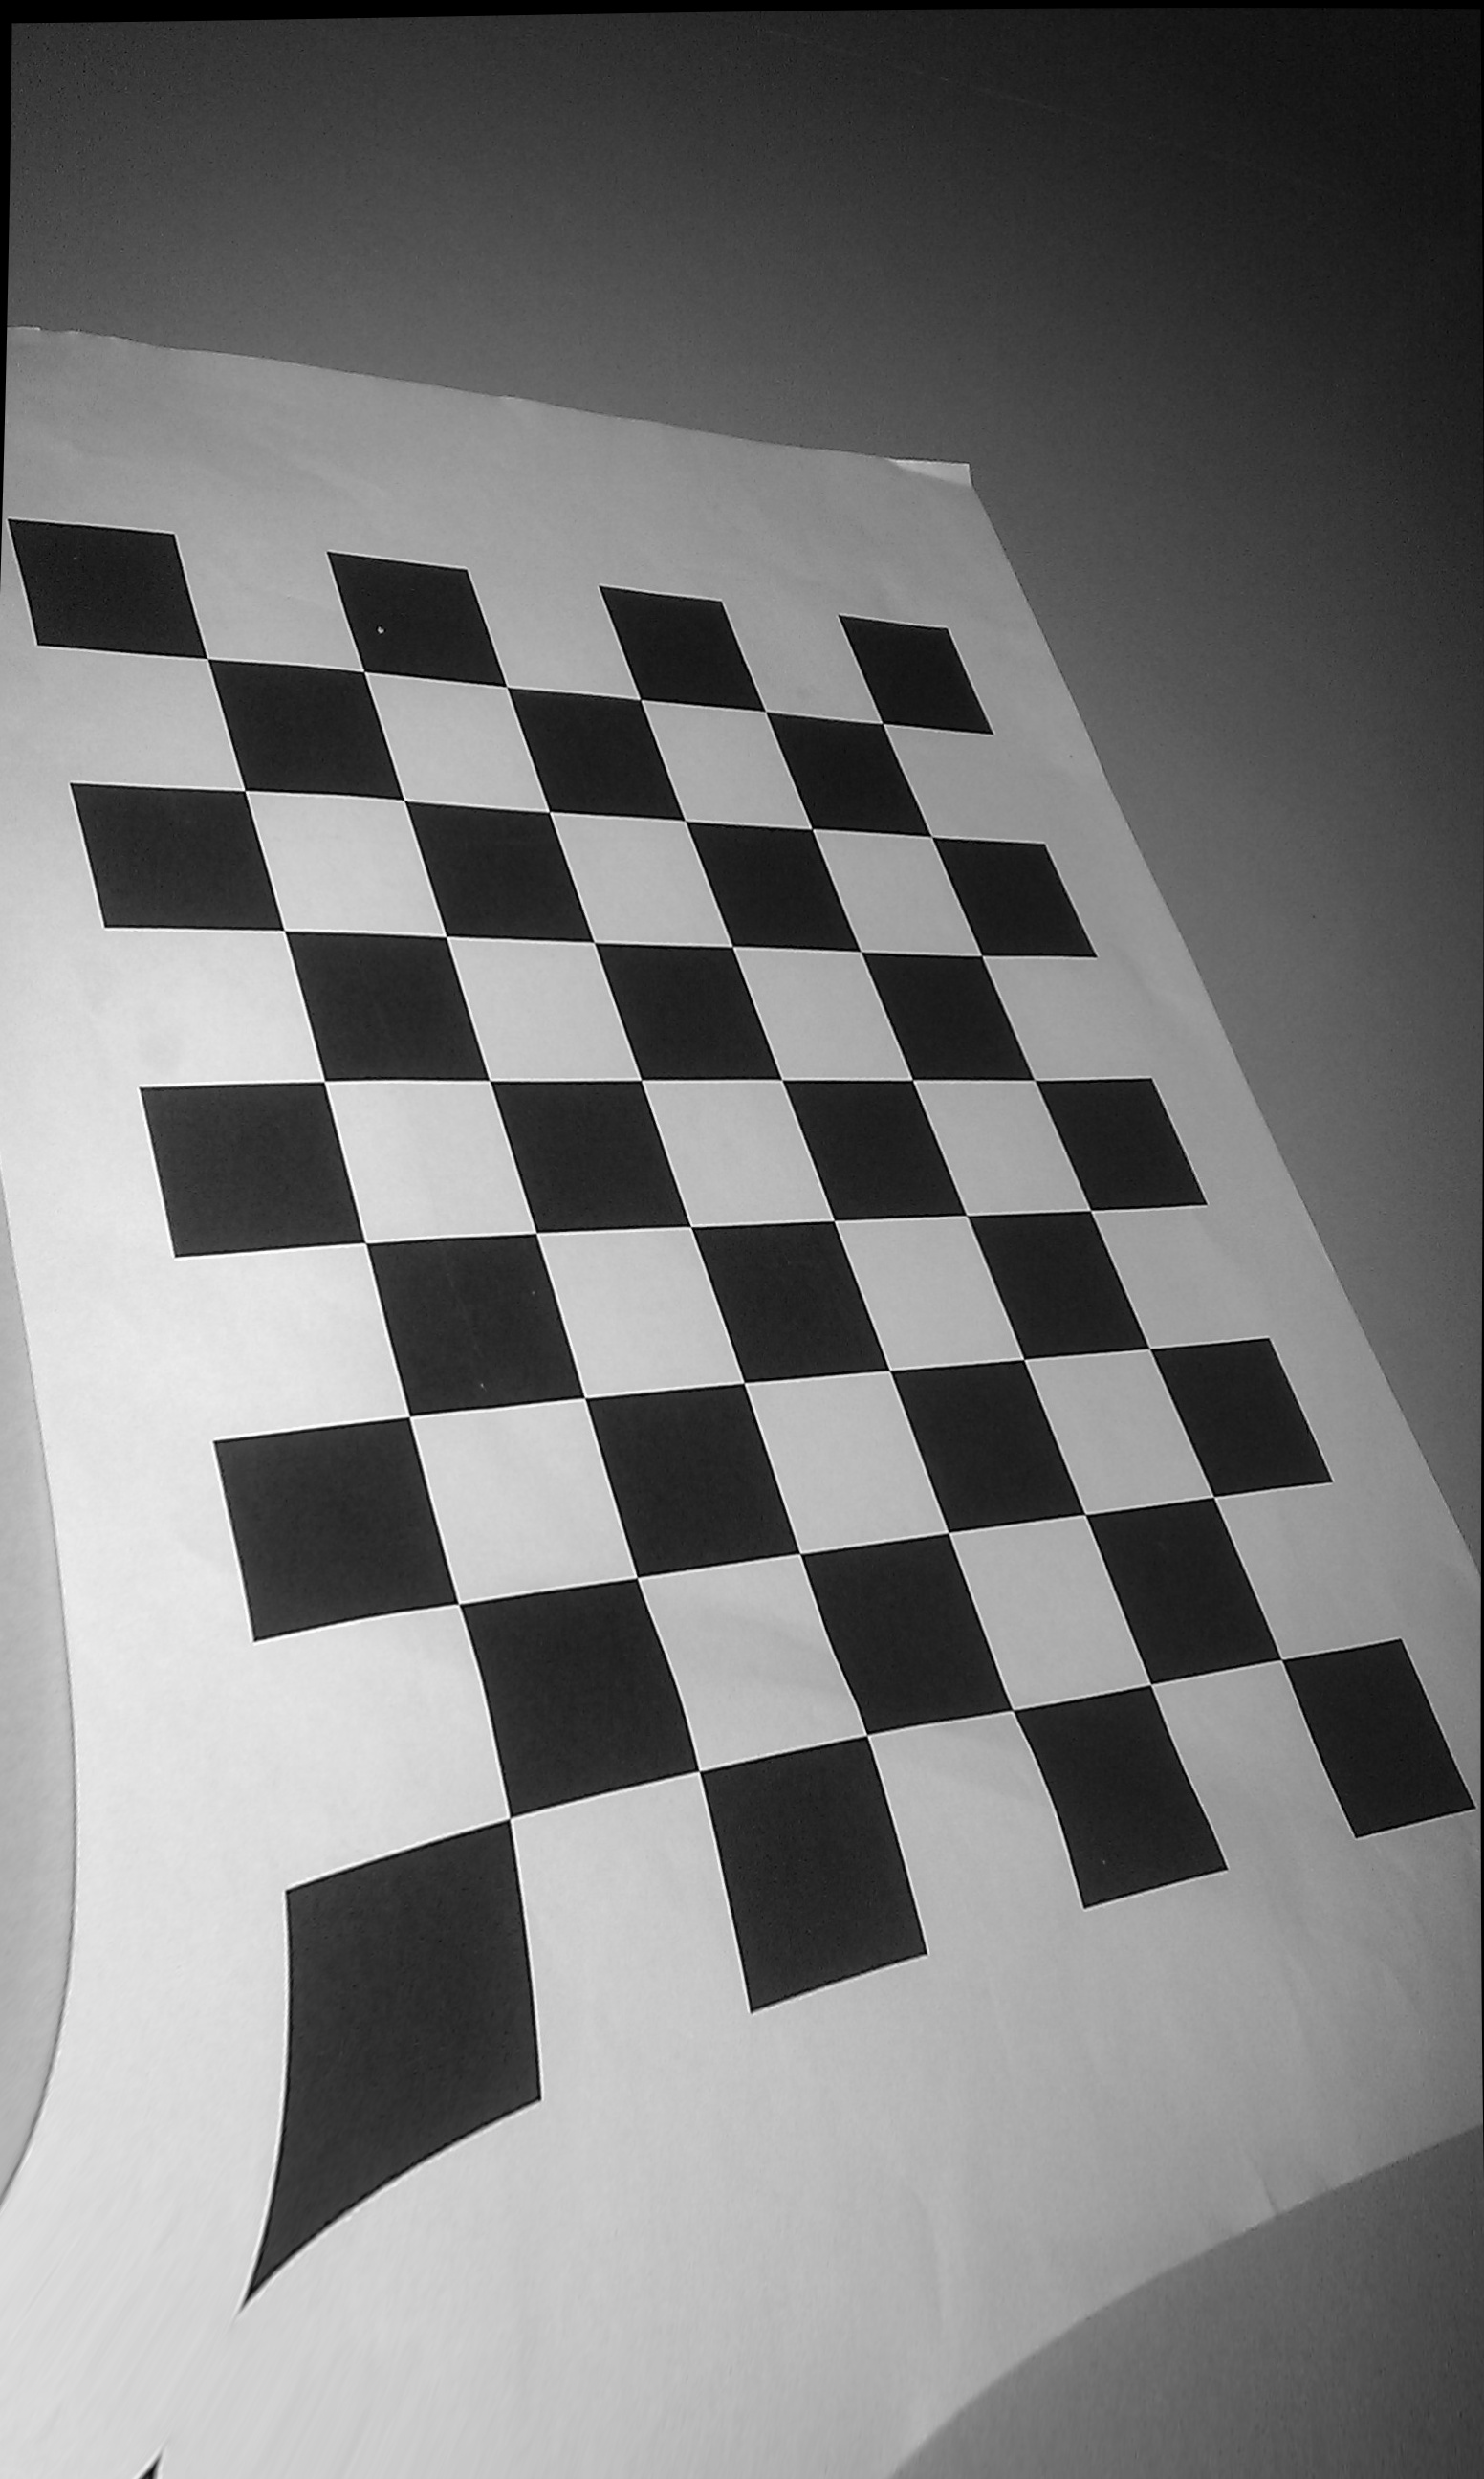
\includegraphics[scale=0.08]{image4.jpg} 
\end{array}$
\end{center}
\caption{The left image is the raw image of the camera.  The right image is the distortet image}
\end{figure}
\section{Part B (Object Detection)}
\subsection{Problem Statement}
In this assignment, the problem of object dection is addressed. This includes distinction between different objects, calculating the centroids and principle angles of the distinct objects and visualizing them in the input image. This is crucial for higher level tasks as grapping the objects with the ER7 arm.

\subsection{Definitions}
Our program takes the path of an image as argument. We refer to it as {\em target image} $I$ and describe it mathematically as $h\times w$-matrix containing grayscale values. A {\em region} $R$ is a set of pixels of the image (i.e.\ $I\subseteq \{(x,y)\in {\mathbb{N}_+}^2| x \leq w \land y\leq h\}$). According to the lecture, the {\em moments} of a region $R$ are
\begin{equation*}
m_{kj} := \sum_{(x,y)\in R} x^ky^j
\end{equation*}
and the {\em central moments} are
\begin{equation*}
\mu_{kj} := \sum_{(x,y)\in R} {(x-x_c)}^k{(y-y_c)}^j
\end{equation*}
where $k,j\in \mathbb{N}_0$ and $(x_c, y_c)$ denotes the centroid of region $R$.

\subsection{Preliminary Considerations}
Suppose there are $n$ objects in the target image. Our implementation conceptually can be divided into three substeps. The first step fetches the following data from the image.

\begin{itemize}
\item The regions $R = \{R_1, R_2,\ldots, R_n\}$ corresponding to the $n$ objects in the image.
\item The moments $m_{00}$, $m_{10}$ and $m_{01}$ for each region.
\item The central moments $\mu_{11}$, $\mu_{20}$ and $\mu_{02}$ for each region.
\end{itemize}

The second step interprets these figures for each region semantically.

\begin{itemize}
\item The moment $m_{00}$ is the number of pixels in the region. We drop regions which are too small -- i.e.\ $m_{00}$ is smaller than a certain threshold $\mathtt{MIN\_REGION\_SIZE}$.
\item The centroid $(x_c,y_c)$ is calculated using the fetched moments [citation needed].
\begin{equation*}
(x_c,y_c) = (\frac{m_{10}}{m_{00}},\frac{m_{01}}{m_{00}})
\end{equation*}
\item The principal angle of the region is [citation needed]
\begin{equation*}
\phi = \frac{1}{2}\cdot \text{arctan2}(2\mu_{11},\mu_{20}-\mu_{02})
\end{equation*}
\end{itemize}

The third step augments the target image with the gained data -- i.e.\ draws a line for each region passing the centroid with the principal angle.

Note that these steps are for illustration purpose only. On implementation level we do not reproduce these steps exactly since they contain backward dependencies (for example we need the centroids from the second step to calculate the central moments) and leave space for performance optimization (for example the regions and the corresponding moments can be build simultaneously).

\subsection{Impementation Process}
The basic process of the implementation is the following:
\begin{enumerate}
\item Prepare image for region detection
\item Search for the regions
\item Calculate centroid and principle angle
\item Augment image
\end{enumerate}

As a note, any function names starting with <cv> are functions provided by the opencv library.

In the first step, the opencv functions cvSmooth, cvThreshold, cvErode and cvDilate are used (in this order).  The cvSmooth function uses a Gaussian Smoothing to remove noise and details.  The function cvThreshold creates a binary image, so that either a pixel is white or black.  The cvErode and cvDilate functions are used to perform an opening operation on the image.  This removes hairlines and restores the objects.

The second step is represented by the "getRegions function". It iterates through all the pixels of an image in order to detect the regions.  White pixels are pixels of objects while black regions are the background.  Therefore all black regions can be ignored.  If the pixel is a white pixel (represents the seed pixel), the function cvFloodFill is used to detect all pixels with the same color connected to the seed pixel.  If the number of pixels exceeds the defined $\mathtt{MIN\_REGION\_SIZE}$ threshold, it is considered a viable region and all the contained pixels are given the color 255 - NumberOfRegions.  Otherwise all the pixels are colored black.  The recoloring is needed, so that if a later pixel of the same region is found, we know in which region to add it.  After this process, the result is a list of regions, each containing a list of its pixels, the number of pixels (size) and the sum of the x and y coordinates. 

The third step is to calculate the centroid and principle angle of each region.  These functions are defined in the Region class.  These functions are based on the formula given in the previous section.

The last step is to visualize the centroids and there corresponding principle angles.  In order to visualize anything, the image needs to be converted to a color image which is done with the cvCvtColor function.  Visualizing the centroid is fairly easy and is achieved by using the cvCircle function.  Displaying the principle angle is more difficult, as some calculations need to be done.  As the principle angle is visualized by using a straight line, we need to calculate the slope of such a line.  The slope can be calculated from the principle angle, by taking the tan of the angle.  However, the principle angle needs to be increased by 90 degrees, as the principle angle is the angle along the y axis, however to calculate slope of the line, we need the angle based on the x axis. In our coordinate system, the x axis is represented by the width of the image, the y axis is along the height of the image.   After this step, the intersection points with the y and x axis are calculated.  A line is drawn between these points using the cvLine function.


\subsection{Result}
The program was able to detect the centroids and principal angle of each object in the given images and visualize these on the source image.  
\end{document}